\section{Metodología de Gestión de Proyectos}
Synaptix adopta PMBOK como marco de dirección, conforme al artículo 4.3 y RT-19.01, y lo aplica mediante una oficina de gestión del proyecto. El enfoque híbrido combina líneas base y control formal de compromisos con ciclos de revisión de productos de dos semanas. La adaptación responde a los hitos contractuales, las dependencias físicas, la operación estacional y la validación de procesos con las personas usuarias. El procedimiento de adaptación de PMI orienta la selección y el ajuste del enfoque; las reglas operativas siguientes corresponden a la propuesta de Synaptix. \parencites[art.~4.3, pp.~5--6]{sd6-ba}[RT-19.01, p.~33]{sd6-bt}[pp.~1--7]{sd6-pmi-adaptacion}

\subsection{Enfoque aplicado y líneas base}
El componente predictivo gobierna alcance, dependencias, adquisiciones, instalación, migración y certificación de etapas. La revisión iterativa permite validar reglas e interfaces antes de completar su construcción, dentro del alcance comprometido. Cada ciclo selecciona resultados verificables según prioridad, dependencias y capacidad disponible; su revisión alimenta la planificación y registra las observaciones. Los ciclos de dos semanas son una cadencia interna: sus resultados se consolidarán para el Comité de Proyecto quincenal, y la validación con personas usuarias se convocará según el producto, la decisión requerida y las ventanas operacionales. Las restricciones del caso prevalecerán sobre el calendario del ciclo. La aceptación contractual y la autorización de producción conservan sus procedimientos propios. \parencite{sd6-pmi-hibrido}

El Jefe de Proyecto dirigirá la oficina y consolidará alcance, requisitos, cronograma, recursos, calidad, riesgos, comunicaciones, interesados y adquisiciones. La oficina se organizará con los responsables del equipo, mediante funciones y suplencias documentadas; cada responsable aportará el estado y la evidencia de su ámbito. Un registro maestro versionado vinculará los requisitos de SD2 y T-12 con el alcance por etapa y los criterios CA-01 a CA-25 de SD3, los entregables y los paquetes de SD7, y las pruebas y actas correspondientes. T-12, el tablero y los informes remitirán a ese registro y a sus evidencias. Se conservarán los identificadores vigentes y la versión de cada fuente. Las diferencias entre documentos se registrarán con responsable y resolución antes de aprobar la línea base afectada. Una declaración de cumplimiento del T-12 deberá acompañarse de su localizador documental y evidencia prevista; no acredita por sí sola una prueba realizada. \parencites[secs.~3.1.2 y 3.2.4, pp.~7--11 y 19--22]{sd6-sd3}[cap.~19, pp.~143--145]{sd6-t12}

El enunciado, la EDT y su diccionario establecerán entregables, criterios de aceptación y responsables; la red y el calendario identificarán dependencias, ruta crítica y holguras. SD7 desarrollará las estimaciones por paquete y su aplicación de PERT y CPM. El esfuerzo se distribuirá entre personas y actividades sin contabilizarlo dos veces, y una duración estimada no se presentará como probabilidad de entrega sin fundamento. Las líneas base de alcance, programación y costo se someterán a aprobación y quedarán versionadas; su formulación en la oferta no acredita la aprobación del cliente. Los valores económicos se mantendrán en el expediente autorizado correspondiente. \parencites[RT-19.03--05, p.~33]{sd6-bt}[arts.~50.2 y 72, pp.~29 y 38]{sd6-ba}

La planificación respetará E1 en los meses 1--16, E2 en 13--21 y Operación en 21--56. En 13--15 coexistirán marcha blanca de E1 y construcción de E2; en 19--20, marcha blanca de E2 y preparación del servicio. Antes de comprometer cada ciclo se comprobarán las horas disponibles y comprometidas por persona y período en todos sus frentes, incluidos comités, validaciones, soporte y transferencia; un recurso compartido no contará como dos personas. La aceptación de la plataforma en el mes 21 se distinguirá de la evaluación del beneficio y transferencia de IN-02, que siguen el calendario de su piloto de invernada. Esta distinción no postergará las funciones, pruebas ni criterios de aceptación exigibles en el mes 21. \parencite[sec.~3.1.2, pp.~7--11]{sd6-sd3}

Para reducir la dependencia de la única persona que opera el sistema heredado, Synaptix iniciará el levantamiento y la transferencia de conocimiento en los primeros ciclos de implementación que dispongan de una ventana admisible. Datos y Funcional documentarán procedimientos, fuentes y mapeo de saldos, coordinarán con el cliente los accesos y respaldos autorizados y programarán la participación de la persona experta y de quien deba reproducir los procedimientos. El mes 6 se conservará como hito de verificación: extracción reproducible, documentación disponible y primer simulacro de cierre en paralelo con conciliación de saldos y diferencias registradas. El Jefe de Proyecto comprobará productos y resultados; desde su incorporación, Operación/SRE participará en la preparación de la continuidad. Synaptix establece este hito como medida preventiva propia, que se integrará en la planificación de alcance, migración, recursos y riesgos. El riesgo residual permanecerá en seguimiento mientras subsista la dependencia, aun cuando se complete la transferencia prevista. \parencites[RT-05.15, p.~34]{sd6-c07}[sec.~3.1.2.1, p.~8]{sd6-sd3}

\subsection{Gobierno, interesados y comunicaciones}
El Jefe de Proyecto tendrá dedicación exclusiva durante toda la implementación y facultades para comprometer a Synaptix en materias de ejecución. La Contraparte Técnica del cliente validará entregables, aprobará avances técnicos, coordinará pruebas y emitirá conformidades; el Administrador del Contrato supervisará el cumplimiento contractual, los estados de pago y las modificaciones. Los responsables de Arquitectura, Seguridad, Datos, Desarrollo, Funcional, Calidad y Pruebas, Integración, Operación e Implantación aportarán decisiones y evidencias dentro de sus competencias. La nómina, certificaciones, experiencia y acreditaciones se documentarán en SD12/T-8, y la dedicación por actividad en SD7/T-15. \parencites[art.~70, p.~37]{sd6-ba}[RT-19.02 y sec.~19.2, pp.~33--34]{sd6-bt}

Los líderes de Desarrollo y Funcional tendrán dedicación del 100\,\% en implementación; los líderes de Datos e Integración, participación permanente durante esa fase. El Arquitecto de Solución tendrá dedicación alta durante el diseño y participación permanente en el Comité de Arquitectura; Seguridad y Calidad y Pruebas mantendrán la participación permanente exigida. El Líder de Operación/SRE se incorporará desde el mes 6 y permanecerá durante Operación, aportando criterios de continuidad, preparación del servicio y transferencia. El Líder de Implantación y Gestión del Cambio se incorporará desde el mes 8 y coordinará preparación de olas, convivencia, capacitación y adopción. La planificación comprobará estos mínimos contra las cargas y períodos de participación, sin confundir la incorporación de un rol con el inicio de un comité o de la fase de servicio. \parencite[sec.~19.2, pp.~33--34]{sd6-bt}

El Jefe de Proyecto conservará la dirección de la implementación y sus responsabilidades hasta la recepción y transferencia correspondientes. Desde el inicio de Operación en el mes 21, el Gerente de Servicio institucional previsto en SD3 coordinará la gestión del servicio y consolidará sus informes, riesgos, cambios y compromisos, con el Líder de Operación/SRE como responsable del seguimiento técnico de la operación. La transición registrará la recepción de documentación y registros, los pendientes con responsable y plazo y las suplencias. La participación posterior del Jefe de Proyecto se declarará con sus funciones y dedicación en SD12/T-8 y SD7/T-15; las responsabilidades contractuales y los participantes obligatorios de los comités se mantendrán. Este relevo organiza el servicio sin presumir una dedicación exclusiva del Jefe de Proyecto durante toda la Operación. \parencites[art.~70, p.~37]{sd6-ba}[sec.~3.1.2.3, pp.~10--11]{sd6-sd3}

La Tabla~\ref{tab:sd6-gobierno} establece las instancias de asistencia obligatoria para ambas partes. La oficina preparará cada sesión con estado de compromisos, decisiones requeridas, alternativas e impactos. El Jefe de Proyecto coordinará la emisión de las actas dentro de los dos días hábiles siguientes, registrando acuerdos, responsables y plazos, y mantendrá seguimiento de su cierre.
\begin{table}[htbp]
\caption{Cadencias y participantes del gobierno del proyecto}\label{tab:sd6-gobierno}
\begin{tabularx}{\linewidth}{L{.21\linewidth}L{.17\linewidth}Y}
\hline
\EncabezadoTabla{Instancia} & \EncabezadoTabla{Frecuencia} & \EncabezadoTabla{Participantes y decisión principal}\\\hline
\rowcolor{SynSurface} Comité Ejecutivo & Mensual & Patrocinador del cliente, gerencia de Synaptix y Administrador del Contrato: decisiones estratégicas, escalamiento, cambios de alcance y riesgos mayores.\\\hline
Comité de Proyecto & Quincenal & Contraparte Técnica y Jefe de Proyecto: cronograma, entregables, desviaciones, riesgos y decisiones operativas.\\\hline
\rowcolor{SynSurface} Comité de Arquitectura & Mensual & Arquitecto de Solución, Encargado de Seguridad y referentes técnicos del cliente: decisiones de arquitectura, deuda y riesgos técnicos.\\\hline
Comité de Operación & Mensual desde mes 13 & Líder de Operación, mesa de servicio y Contraparte Técnica: niveles de servicio, incidentes, problemas y mejora continua.\\\hline
\rowcolor{SynSurface} Reunión de seguimiento & Semanal & Equipos de ambas partes: coordinación operativa, impedimentos y compromisos de la semana.\\\hline
\end{tabularx}
\FuenteTabla{Bases Administrativas, art.~71, pp.~37--38; Bases Técnicas Transversales, RT-19.04/09, pp.~33--34.}
\end{table}
Estas instancias distinguen la revisión técnica de la autorización contractual. Su convocatoria, participantes, entradas, productos y seguimiento se documentarán en el Formulario T-9, \ArchivoTNueve. El inicio del Comité de Operación en el mes 13 prepara el servicio y la transición, con el Líder de Operación/SRE ya incorporado desde el mes 6, sin adelantar la fase contractual de Operación de los meses 21--56.

El registro de interesados identificará proceso, autoridad de decisión, impacto, disponibilidad, suplencia y canal de comunicación. La Contraparte Técnica coordinará validaciones con administración, torre, portería, varadero y escuela; el responsable funcional de Synaptix consolidará observaciones y resolverá o escalará conflictos. Las sesiones agruparán tareas y usarán ventanas compatibles con turnos y faenas. Cada convocatoria anticipará el producto, los criterios, las preguntas o pruebas y la decisión requerida; su esfuerzo se estimará por perfil, actividad y período, incluyendo preparación y revisión. La oficina distinguirá la dedicación a administración funcional de la requerida para comités, pruebas y aceptación; el límite de esfuerzo funcional previsto en SD3 para Operación no se utilizará como presupuesto universal de participación del cliente. La ausencia de un área TI en la marina no elimina estas responsabilidades ni convierte a su dotación de invierno en un equipo informático permanente. El plan de adopción por perfil se desarrolla en SD3; aquí se gobiernan su programación, responsables y evidencia. \parencites[numerales 13.1--13.3, pp.~28--30]{sd6-c07}[secs.~3.1.2.3 y 3.4.4, pp.~10--11 y 31--32]{sd6-sd3}

Synaptix habilitará un espacio colaborativo accesible al cliente con documentación, entregables, actas, riesgos y cambios actualizados. Cada registro identificará responsable, versión, fecha y estado; la oficina incorporará los acuerdos y enlazará los documentos afectados. El plan de comunicaciones de T-9 vinculará cada producto con emisor, destinatario, canal, frecuencia o disparador, decisión requerida y constancia de recepción cuando corresponda. Los accesos se asignarán por función, evitando exponer antecedentes de salud, menores o expedientes personales a participantes que no los requieran. El tablero del proyecto permanecerá accesible al cliente en cualquier momento. \parencite[RT-19.05/08, pp.~33--34]{sd6-bt}

\subsection{Control integrado de cambios y adquisiciones}
Cada observación se registrará y clasificará como defecto, precisión dentro del alcance o modificación de un compromiso contractual. El Jefe de Proyecto registrará el fundamento de la clasificación con apoyo de los responsables funcionales, técnicos y de calidad que correspondan; durante Operación, el Gerente de Servicio coordinará ese registro dentro de sus atribuciones. La corrección de un defecto y la precisión conservarán las obligaciones y los criterios de recepción. Si la propuesta modifica un compromiso, se abrirá una solicitud formal y se evaluará su impacto en alcance, plazo, costo, riesgo y niveles de servicio, conforme al artículo 72.

\newpage 
La Figura~\ref{fig:control_cambios} distingue la corrección dentro del alcance del procedimiento de modificación contractual, e identifica las condiciones que deben cumplirse antes de ejecutar un cambio.

\begin{figure}[htbp]
    \centering
    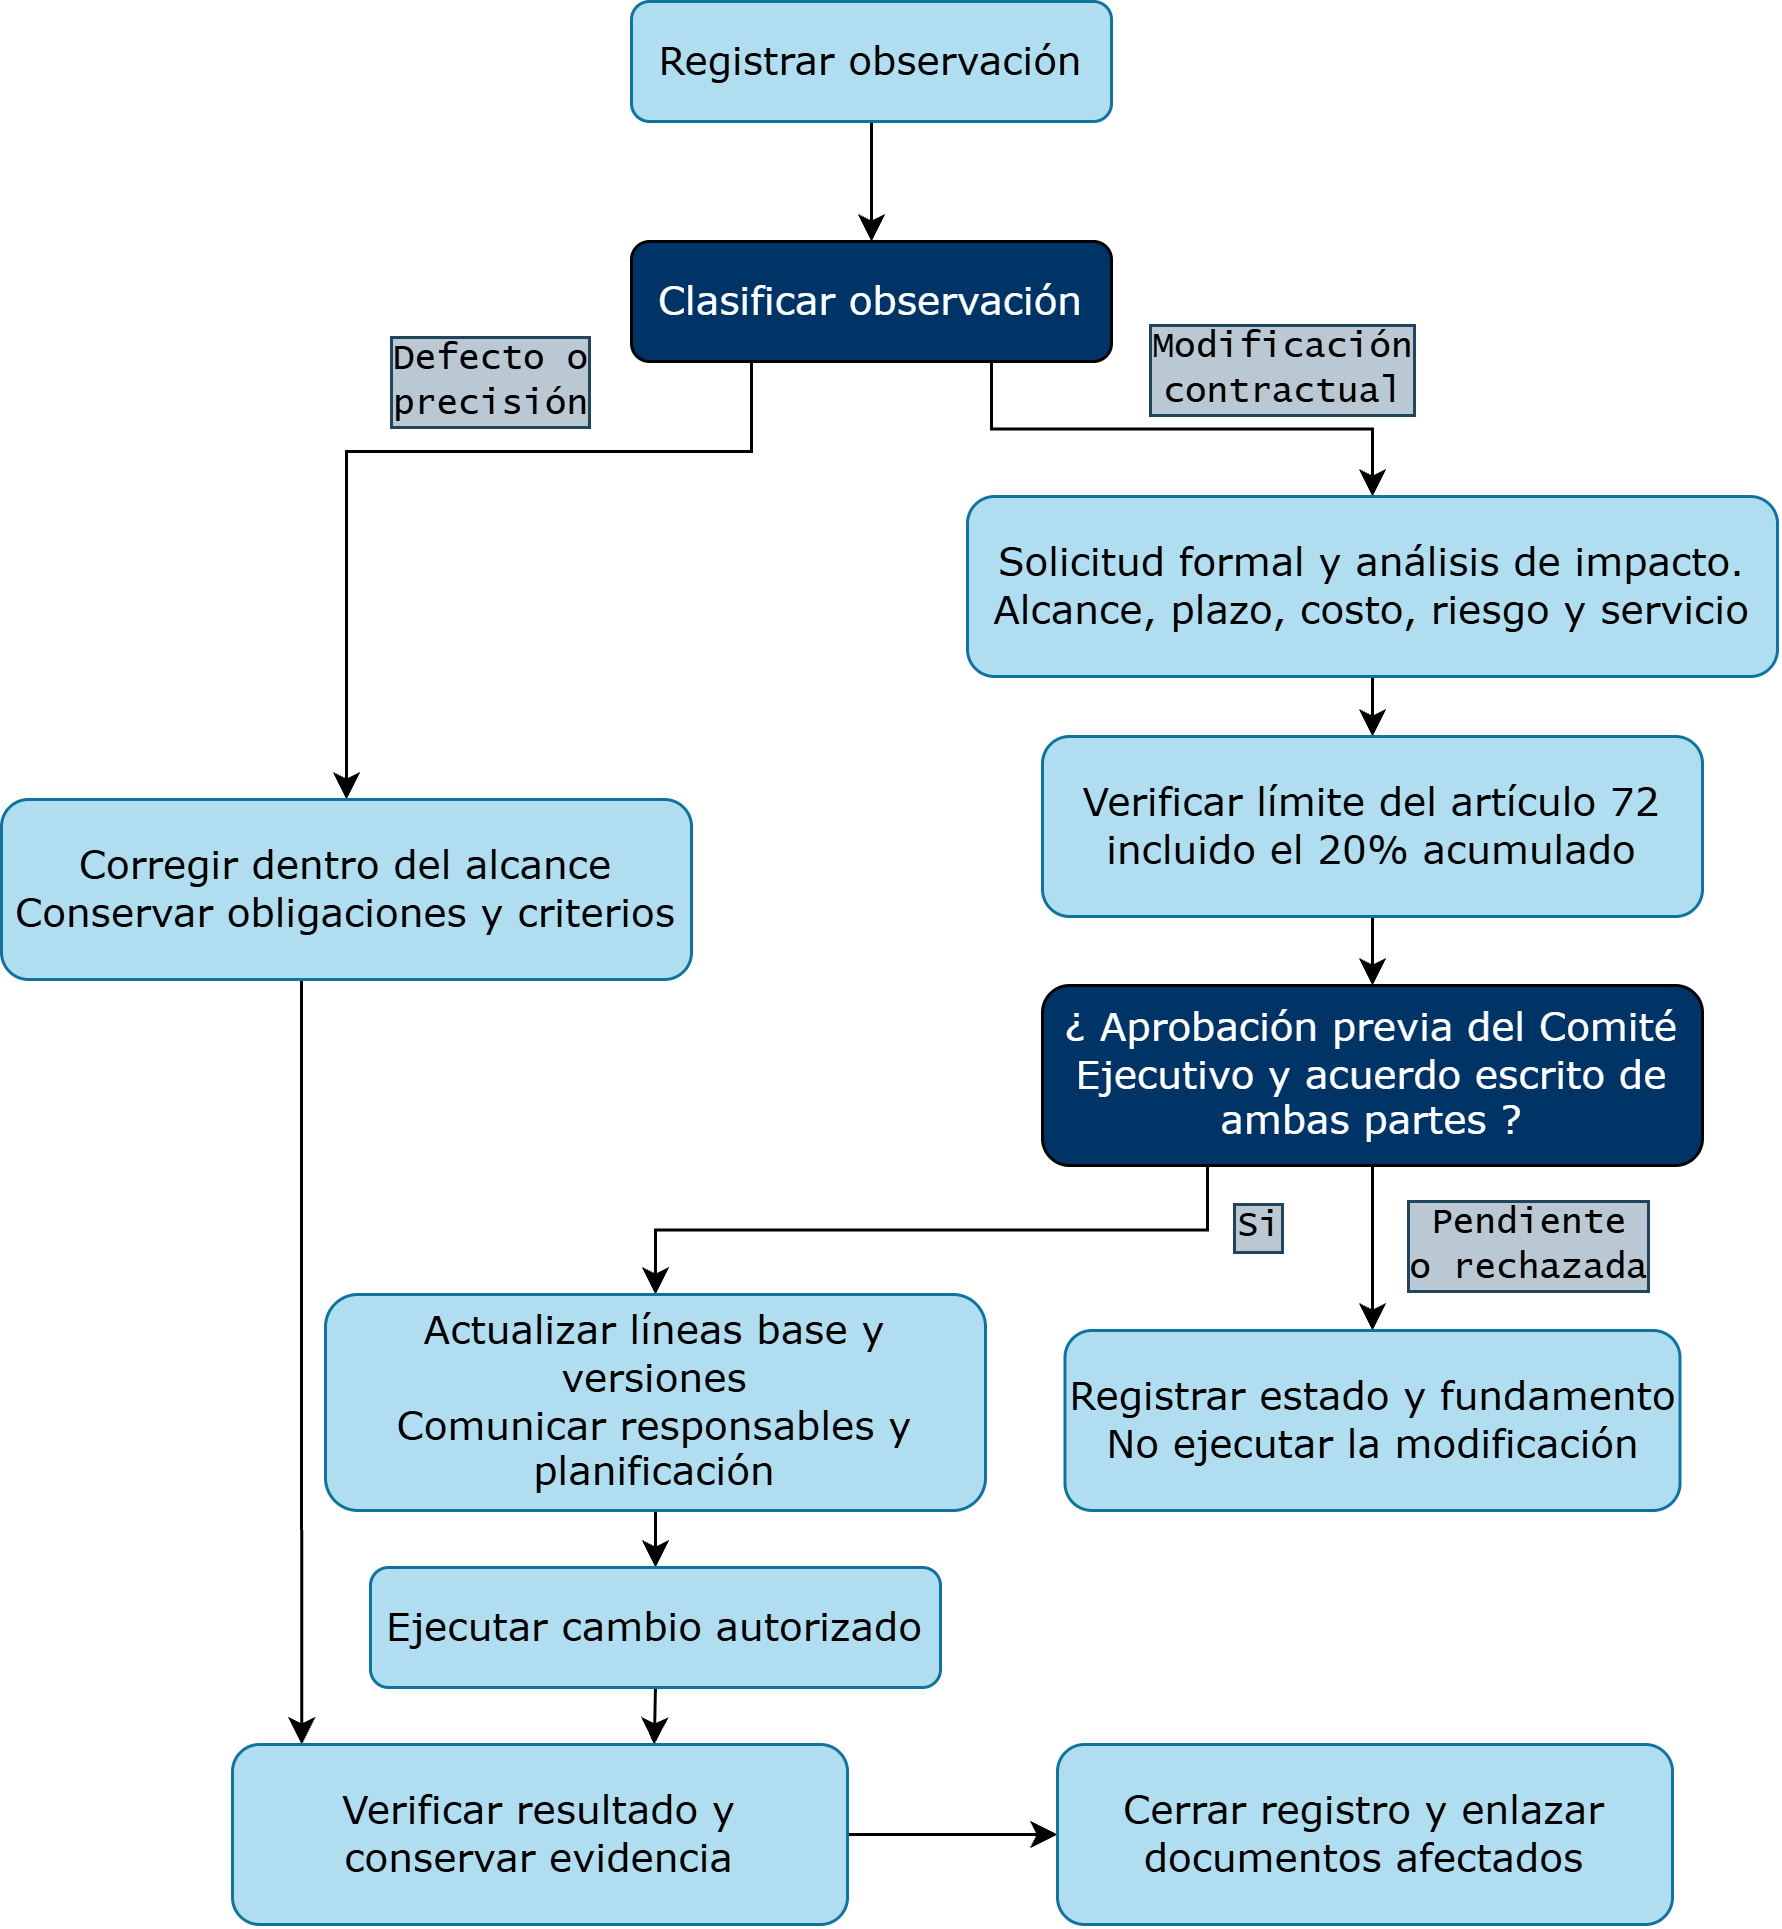
\includegraphics[width=0.8\linewidth]{figuras/F6_1.png}
    \caption{Procedimiento de control integrado de cambios}
    \label{fig:control_cambios}
    \par\fontsize{9}{12}
\end{figure}

La solicitud identificará origen, justificación, documentos afectados, alternativas, impactos y recomendación. El Comité Ejecutivo aprobará el cambio antes de ejecutarlo y ambas partes lo formalizarán por escrito. Se comprobarán el límite acumulado del 20\,\% del valor original del Contrato y la prohibición de modificar su objeto principal, naturaleza, garantías mínimas o cronograma obligatorio del artículo 17. 

Una vez autorizado, el Jefe de Proyecto actualizará las líneas base y comunicará la versión aplicable; tras la ejecución se verificará el resultado y se cerrará el registro. Una solicitud pendiente o rechazada no habilitará su ejecución. Los importes del análisis permanecerán fuera de la oferta técnica.

Las adquisiciones se vincularán a paquetes, dependencias y fechas de necesidad de SD7 y al inventario T-11. Conforme al capítulo 11 del Caso 07, el cliente ejecutará las obras físicas requeridas, incluidas canalizaciones, obras eléctricas, torretas y postación, y adquirirá el hardware que el caso le asigna: medidores, lectores de credencial, dispositivos de terreno, instrumentación del surtidor y equipamiento de red. Synaptix especificará qué comprar, cuánto y con qué características, y considerará esas dependencias en diseño, integración, programación y riesgo. El registro distinguirá esta frontera exigida por el caso de los bienes y servicios incluidos en la oferta de Synaptix y de los supuestos adicionales de colaboración de SD3. La valorización se mantendrá en el expediente económico correspondiente. \parencites[cap.~11, pp.~26--27]{sd6-c07}[sec.~3.2.2, pp.~15--16]{sd6-sd3}

Para cada dependencia se identificarán responsable de provisión, especificación, fecha de necesidad, plazo de suministro, condición de recepción y respuesta ante atraso. Arquitectura comprobará compatibilidad e interfaces; Seguridad, licencias y tratamiento de datos; y Calidad, evidencia de recepción técnica. La oficina controlará proveedor, producto, sustituciones y riesgo de suministro, y comprobará la disponibilidad de los insumos antes de comprometer la instalación o prueba afectada. Un supuesto adicional no se utilizará como exención automática de una obligación de las bases. La justificación de hacer o comprar y las condiciones de subcontratación se desarrollarán en SD12. Toda subcontratación requerirá autorización previa y escrita del cliente y la verificación de los límites y condiciones del artículo 73, sin presumir contratos o autorizaciones obtenidos. \parencite[arts.~71--73, pp.~37--38]{sd6-ba}

\subsection{Seguimiento cuantitativo y respuesta a desviaciones}
Synaptix emitirá un informe mensual con estado del cronograma, avance físico y financiero, entregables del período, desviaciones, riesgos, incidencias y compromisos siguientes. El Jefe de Proyecto consolidará el informe de implementación y el Gerente de Servicio el de Operación, con los responsables y el relevo establecidos en el gobierno del proyecto. El tablero enlazará esos resultados con paquetes, pruebas, actas y decisiones, e identificará fecha de corte y responsable de actualización. El avance se medirá mediante valor ganado: $SPI=EV/PV$ y $CPI=EV/AC$, donde $PV$ es el valor presupuestado del trabajo planificado, $EV$ el del trabajo realizado y $AC$ su costo real. Los tres valores usarán la misma base monetaria y fecha de corte; las horas sin ponderación de costo no sustituirán a $AC$. \parencites[RT-19.06--08, p.~34]{sd6-bt}[p.~1]{sd6-nasa}

Antes de iniciar cada paquete se fijarán su valor planificado, distribución temporal, responsable y regla de reconocimiento de avance. Para productos cuya ejecución esté prevista dentro de un único período mensual de reporte se aplicará la regla 0/100: ningún valor ganado hasta completar y verificar el resultado, y reconocimiento del valor presupuestado al terminarlo. Los paquetes que abarquen varios períodos se descompondrán en hitos intermedios verificables, ponderados según el valor presupuestado del trabajo asociado; las ponderaciones sumarán el total del paquete y cada resultado se reconocerá una sola vez. La distribución del presupuesto se justificará mediante las estimaciones de recursos y costos, sin asignar porcentajes subjetivos por percepción de avance. En cada corte, la oficina respaldará $EV$ con productos y verificaciones y conciliará $AC$ con registros de costo. Para servicios periódicos, el valor se reconocerá contra el resultado verificable del período, sin computar anticipadamente meses futuros. El informe conservará por separado los resultados de calidad y niveles de servicio: un índice de desempeño favorable no acredita su cumplimiento. El avance interno no sustituirá el acta de aceptación del cliente ni habilitará por sí mismo un pago. T-9 documentará estas reglas y SD7 su aplicación a los paquetes.

Los importes se administrarán en el expediente contractual y económico autorizado. SD6 describe el método sin publicar precios, tarifas ni valores que permitan inferir el monto de la oferta, conforme al artículo 50.2. Si un denominador es cero, el índice se declarará no calculable y se explicará la causa. El informe distinguirá avance físico, desempeño de programación, desempeño de costo y estado de aceptación; un índice agregado no reemplazará el control de la ruta crítica. \parencite[art.~50.2, p.~29]{sd6-ba}

Toda desviación superior al 10\,\% en un hito se comunicará dentro de los cinco días hábiles de detectada, con causa, impacto y plan de recuperación, responsable y plazo. Para aplicar de forma reproducible el disparador temporal, Synaptix propone medir la diferencia entre la fecha proyectada y la fecha de término de línea base respecto de la duración planificada del bloque de actividades que conduce al hito:
\[
\Delta_h=100\,\frac{\left|F_h^{p}-F_h^{0}\right|}{F_h^{0}-I_h^{0}}.
\]
Aquí, $F_h^{p}$ es la fecha proyectada de término, $F_h^{0}$ la fecha de término de línea base e $I_h^{0}$ el inicio de referencia del bloque asociado al hito. Las diferencias se expresarán en días corridos. Para todos los hitos se aplicará la misma regla de selección: el bloque comprenderá las actividades específicas de producción, integración, verificación y recepción de los entregables que culminan en ese hito, según la EDT; $I_h^{0}$ será el inicio más temprano de esas actividades en la línea base. No se incorporarán actividades ajenas ni se utilizará automáticamente la duración total del contrato. SD7 identificará el bloque, sus actividades y duración positiva, y T-9 conservará la regla antes de comenzar el seguimiento. Si el hito es instantáneo, se utilizará la duración del bloque asociado; no se dividirá por la duración cero del hito ni se cambiará el bloque durante el seguimiento para reducir el porcentaje. Cada corte mostrará también la fecha prevista, los días de adelanto o atraso y la holgura del cronograma actualizado. Este criterio es una propuesta operativa de Synaptix, sujeta a la aprobación de la línea base; las bases fijan el umbral y el plazo de comunicación, pero no esta fórmula. \parencite[RT-19.10, p.~34]{sd6-bt}

La oficina registrará la primera detección que supere el umbral y calculará desde ella los cinco días hábiles, conservando fecha, versión de línea base, proyección y cálculo. Todo riesgo de incumplir un hito obligatorio se elevará al Jefe de Proyecto desde su detección, aunque todavía no supere el 10\,\%. Se evaluarán fecha prevista, holgura y capacidad, manteniendo el historial; el umbral no autoriza desplazar fechas contractuales. Cualquier modificación contractual seguirá el procedimiento anterior.

La gestión del riesgo seguirá ISO 31000:2018 mediante el plan de SD8 y el registro T-16: contexto, identificación, análisis, evaluación, tratamiento, comunicación y seguimiento. En cada Comité de Proyecto se revisarán riesgos nuevos y abiertos, respuestas, responsables, plazos, disparadores y riesgo residual. Un riesgo materializado se enlazará con la incidencia y su respuesta, conservando el historial. La oficina coordinará los efectos sobre planificación, adquisiciones, calidad y servicio, sin convertir una actualización del registro en autorización para cambiar el contrato. \parencites[RT-19.04, p.~33]{sd6-bt}{sd6-iso31000}

\subsection{Protección de la operación y evidencia de aplicación}
La planificación respetará el congelamiento total del 15 de diciembre al 15 de marzo, la protección del varadero en abril--mayo y septiembre--noviembre, y los congelamientos locales en las 14 fechas náuticas. Ante un aviso de marejadas se suspenderá inmediatamente toda actividad programada del proyecto, incluida la construcción aislada o remota. El Jefe de Proyecto, o el Gerente de Servicio durante Operación, registrará la suspensión, el trabajo afectado, la capacidad y el consumo de reserva; sólo reprogramará tras cesar la condición y comprobar una ventana admisible. SD7 cuantificará y localizará las reservas según exposición, dependencias y ventanas disponibles, con justificación de su estimación; se contabilizarán una sola vez y no autorizarán desplazar hitos contractuales. La atención de una emergencia real seguirá su procedimiento de incidente, sin habilitar trabajo programado. Los mantenimientos programados requerirán aviso al cliente con al menos diez días hábiles. \parencites[cap.~10, restricción 12, p.~26; numeral 13.2, p.~29; cap.~15, RT-10.05, p.~34]{sd6-c07}[art.~20, p.~15]{sd6-ba}[RT-10.05, p.~22]{sd6-bt}

El expediente de gestión vinculará requisito y criterio de aceptación, etapa, entregable, paquete, responsable, prueba, resultado y decisión. Conservará versiones de línea base, comprobaciones de capacidad, actas, riesgos, cambios, aceptaciones e informes. T-9 especificará los campos y responsables de cada registro; T-12 remitirá al apartado y a la evidencia prevista para cada requisito, distinguiendo gobierno del proyecto, arquitectura, desarrollo, pruebas y operación. La aplicación se comprobará mediante el seguimiento de cambios efectivamente tramitados, la reproducción de un corte de valor ganado desde sus registros y la comparación entre carga comprometida y capacidad disponible. Cada evidencia distinguirá lo planificado, lo ejecutado y lo aceptado, sin presentar este procedimiento como resultado ya obtenido.